\subsubsection{Giant Language model Test Room}
\label{sub:gltr}

\gls{gltr}~\footcite{DBLP:journals/corr/abs-1906-04043} is the result of a collaboration of \textit{MIT-IBM Watson AI lab}~\footnote{\url{https://mitibmwatsonailab.mit.edu/}} and \textit{HarvardNLP}~\footnote{\url{http://nlp.seas.harvard.edu/}} with the goal of providing a tool to support non-expert humans in detecting whether a text was generated by a model or not. The authors see many paths for malicious actors to abuse current \gls{lm}s for the purpose of generating fake reviews, comments or news articles and thereby influencing the public opinion. In their work, the authors argue that the \gls{lm}s' ways of working are prone to be detected by simple statistical methods when used as a visual assistance tool. The core assumption is that systems over generate from a restricted subset of the true distribution of natural language, for which they have high confidence. While one might argue that this approach will only be successful if access to the system distribution is provided, Gehrmann and Strobelt hypothesize that these methods generalize well to black-box scenarios, as long as the synthetic text follows a similar sampling strategy than that of a large language model. GLTR assists its users by highlighting sequences that are very probable and unsurprising with green and yellow colors and sequences that are rather unlikely and uncommon with purple and red colors (figure~\ref{fig:gltr}).

\begin{figure}[h]
  	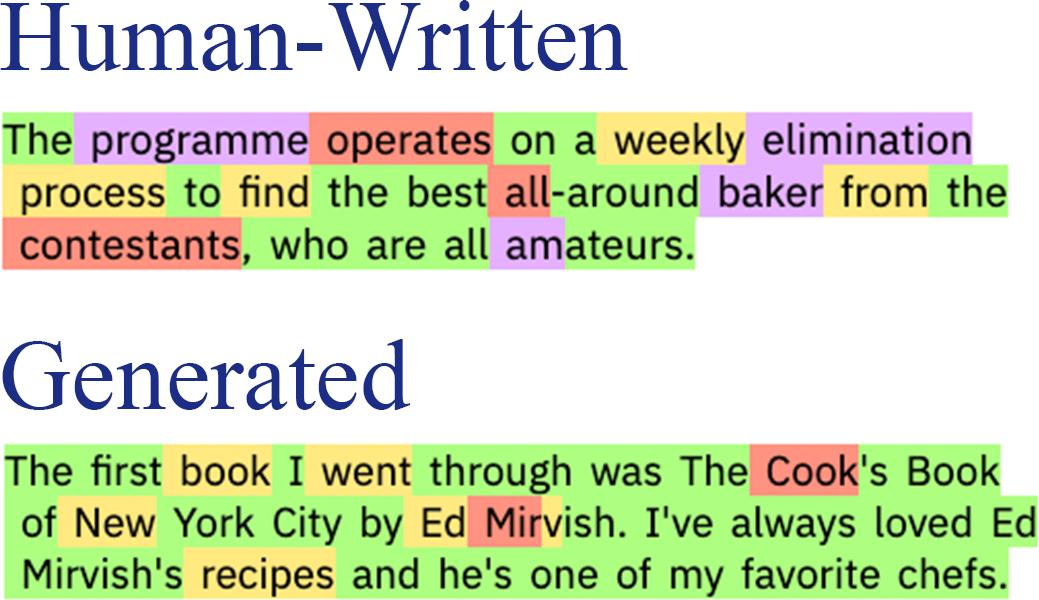
\includegraphics[height=5cm]{img/gltr}
  	\caption[GLTR visualization]{GLTR visualization~\footcite{DBLP:journals/corr/abs-1906-04043}}
	\label{fig:gltr}
\end{figure}

In order to calculate the likelihood of text, \gls{gltr} applies three different tests: \textbf{Test 1} computes the probability of the word $ p_{\text{det}}(X_i = \hat{X}_i | X_{1:i-1}) $. \textbf{Test 2} computes the absolute rank of a word, e.g. rank in $ p_{det}(X_i | X_{1:i-1}) $ and \textbf{test 3} computes the entropy of the predicted distribution, e.g. $ - \sum_w p_{\text{det}}(X_i = w | X_{1:i-1}) \ \text{log} \ p_{\text{det}}(X_i = w | X_{1:i-1}) $. The first two tests check whether a generated word is sampled from the top of the distribution and the third test checks if the preceding context is well-known to the detection system such that it is sure of its next prediction. By default, a word that ranks within the top 10 is highlighted in green, top 100 in yellow, top 1,000 in red, and the rest in purple. The results of a conducted human-subjects study showed that \gls{gltr} improved the human detection-rate of fake text from 54\% to 72\% without any prior training. While an adversarial scheme might try to fool \gls{gltr}, it would be forced to sample from the tail of the distribution and thus risk decreasing coherence of a text which makes it in turn easier for a human to identify the synthetic text. A significant limitation, however, results from the fact that a hidden seed text might be utilized to condition the sample distributions. Then, a conditional distribution will be different, even if \gls{gltr} has access to the model. While \gls{gltr} has this shortcoming, the authors are confident that their tool might be used to e.g. assist moderators on social media or review platforms.
